\chapter{Multiphysics inverse design problems}

Bla bla bla... Brief in formulations (PDEs and couplings), more about uses and applications.

%\begin{figure}[tb]
%    \centering
%    \makebox[\textwidth][c]{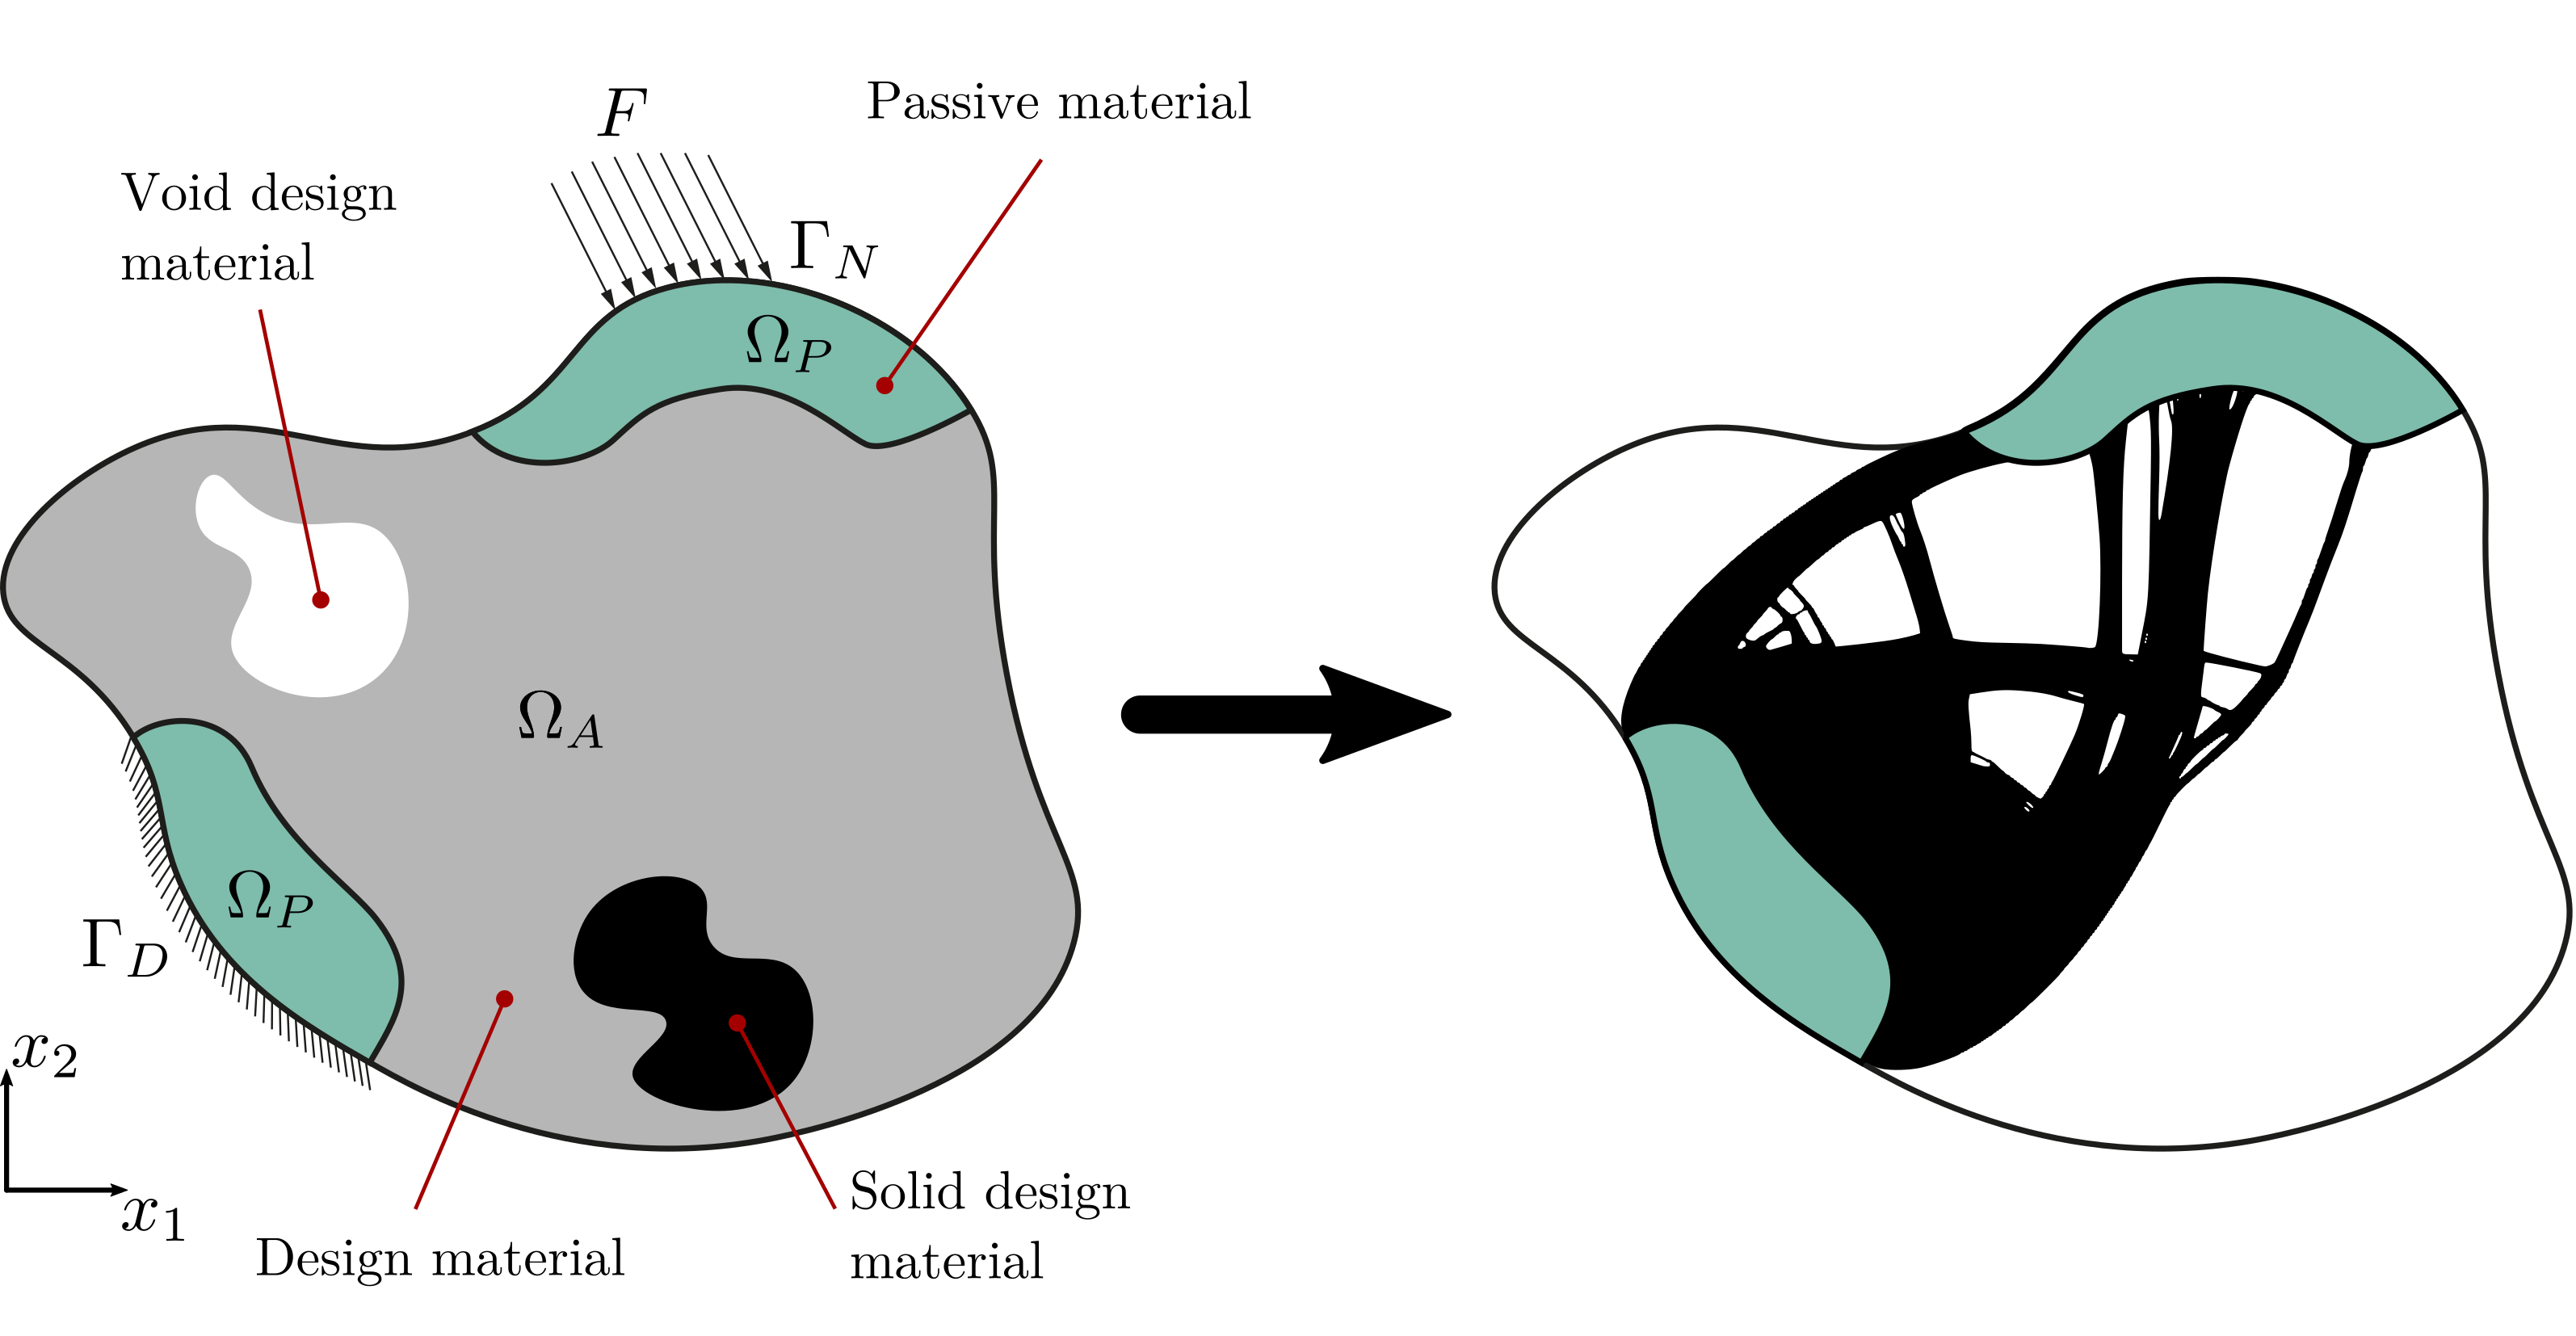
\includegraphics[width=1\imwidth]{figures/simpModel.png}}%
%    \caption{Bla bla bla...}
%    \label{fig:illustateTopOpt}
%\end{figure}


%\begin{equation}
%    (EIu'')'' = q
%\end{equation}


%\begin{figure}[tb]
%    \centering
%    \makebox[\textwidth][c]{\begin{tikzpicture}[remember picture]
    \begin{scope}[xshift=0mm]
        % angle (deg)
        \newcommand\ai{10}
        % line width
        \newcommand\wi{1pt}
        % cell size
        \newcommand\cellsize{3}
        % Rank-$N$ size
        \newcommand\di{0.75}

        % cell
        \draw[gray!10,   fill=gray!10, rotate around={\ai:(0,0)}] (0,0) rectangle (\cellsize,\cellsize) node (rect1) {};
        \draw[black!60, fill=black!60, rotate around={\ai:(0,0)}] (0,0) rectangle (\di,\cellsize);

        % orientation frame
        \draw[black, -stealth, line width=\wi, rotate around={\ai:({\di*cos(\ai) - \cellsize/2*sin(\ai)},{\di*sin(\ai) + \cellsize/2*cos(\ai)})}] ({\di*cos(\ai) - \cellsize/2*sin(\ai)},{\di*sin(\ai) + \cellsize/2*cos(\ai)}) -- ({\di*cos(\ai) - \cellsize/2*sin(\ai) + 0.75},{\di*sin(\ai) + \cellsize/2*cos(\ai)});
        \draw[black, -stealth, line width=\wi, rotate around={\ai:({\di*cos(\ai) - \cellsize/2*sin(\ai)},{\di*sin(\ai) + \cellsize/2*cos(\ai)})}] ({\di*cos(\ai) - \cellsize/2*sin(\ai)},{\di*sin(\ai) + \cellsize/2*cos(\ai)}) -- ({\di*cos(\ai) - \cellsize/2*sin(\ai)},{\di*sin(\ai) + \cellsize/2*cos(\ai) + 0.75});

        % local frame
        \draw[black, -stealth, dashed, line width=\wi] (0,0) -- ({\cellsize + 0.8},0);
        \draw[black, -stealth, dashed, line width=\wi] (0,0) -- (0,{\cellsize + 0.8});

        % ruler
        \draw[black, |-|, line width=\wi, rotate around={\ai:(0,0)}] (0,0) -- (\cellsize,0);
        \draw[black,  -|, line width=\wi, rotate around={\ai:(0,0)}] (0,0) -- (\di,0);

        % arc
        \draw[black, dotted, line width=\wi] (\cellsize,0) arc (0:\ai:\cellsize);

        % annotation
        \draw (\cellsize + 0.7, -0.3) node {$x_1 / \epsilon^3$};
        \draw (-0.5, \cellsize + 0.8) node {$x_2 / \epsilon^3$};
        \draw (\cellsize/2,-0.75) node {Rank-$1$};

        \draw[rotate around={{\ai/2}:(0,0)}] ({\cellsize+0.3},0) node {$\theta_1$};

        \draw[rotate around={{\ai}:(0,0)}] ({\di/2},0.4) node [rotate around={{\ai}:(0,0)}] {$\mu_1$};
        \draw[rotate around={{\ai}:(0,0)}] ({(\cellsize - \di)/2 + \di},0.4) node [rotate around={{\ai}:(0,0)}] {$1-\mu_1$};

        \draw[rotate around={{\ai}:(0,0)}] ({0+0.4},{\cellsize-0.4}) node [rotate around={{\ai}:(0,0)}] {$(+)$};
        \draw[rotate around={{\ai}:(0,0)}] ({\cellsize-0.4},{\cellsize-0.4}) node [rotate around={{\ai}:(0,0)}] {$(-)$};
        \coordinate (A) at (rect1.north);


        \draw[rotate around={\ai:({\di*cos(\ai) - \cellsize/2*sin(\ai)},{\di*sin(\ai) + \cellsize/2*cos(\ai)})}] ({\di*cos(\ai) - \cellsize/2*sin(\ai)+1} , {\di*sin(\ai) + \cellsize/2*cos(\ai) + 0.2}) node {$\mathbf{n}_1$};
        \draw[rotate around={\ai:({\di*cos(\ai) - \cellsize/2*sin(\ai)},{\di*sin(\ai) + \cellsize/2*cos(\ai)})}] ({\di*cos(\ai) - \cellsize/2*sin(\ai) + 0.3} , {\di*sin(\ai) + \cellsize/2*cos(\ai) + 1}) node {$\mathbf{m}_1$};



    \end{scope}
    \begin{scope}[xshift=45mm]
        % angle (deg)
        \newcommand\ai{15}
        % line width
        \newcommand\wi{1pt}
        % cell size
        \newcommand\cellsize{3}
        % Rank-$N$ size
        \newcommand\di{0.6}

        % cell
        \draw[gray!40,   fill=gray!40, rotate around={\ai:(0,0)}] (0,0) rectangle (\cellsize,\cellsize) node (rect2) {};
        \draw[black!60, fill=black!60, rotate around={\ai:(0,0)}] (0,0) rectangle (\di,\cellsize);

        % orientation frame
        \draw[black, -stealth, line width=\wi, rotate around={\ai:({\di*cos(\ai) - \cellsize/2*sin(\ai)},{\di*sin(\ai) + \cellsize/2*cos(\ai)})}] ({\di*cos(\ai) - \cellsize/2*sin(\ai)},{\di*sin(\ai) + \cellsize/2*cos(\ai)}) -- ({\di*cos(\ai) - \cellsize/2*sin(\ai) + 0.75},{\di*sin(\ai) + \cellsize/2*cos(\ai)});
        \draw[black, -stealth, line width=\wi, rotate around={\ai:({\di*cos(\ai) - \cellsize/2*sin(\ai)},{\di*sin(\ai) + \cellsize/2*cos(\ai)})}] ({\di*cos(\ai) - \cellsize/2*sin(\ai)},{\di*sin(\ai) + \cellsize/2*cos(\ai)}) -- ({\di*cos(\ai) - \cellsize/2*sin(\ai)},{\di*sin(\ai) + \cellsize/2*cos(\ai) + 0.75});

        % local frame
        \draw[black, -stealth, dashed, line width=\wi] (0,0) -- ({\cellsize + 0.8},0);
        \draw[black, -stealth, dashed, line width=\wi] (0,0) -- (0,{\cellsize + 0.8});

        % ruler
        \draw[black, |-|, line width=\wi, rotate around={\ai:(0,0)}] (0,0) -- (\cellsize,0);
        \draw[black,  -|, line width=\wi, rotate around={\ai:(0,0)}] (0,0) -- (\di,0);

        % arc
        \draw[black, dotted, line width=\wi] (\cellsize,0) arc (0:\ai:\cellsize);

        % annotation
        \draw (\cellsize + 0.7, -0.3) node {$x_1 / \epsilon^2$};
        \draw (-0.5, \cellsize + 0.8) node {$x_2 / \epsilon^2$};
        \draw (\cellsize/2,-0.75) node {Rank-$2$};

        \draw[rotate around={{\ai/2}:(0,0)}] ({\cellsize+0.3},0) node {$\theta_2 + \pi/4$};

        \draw[rotate around={{\ai}:(0,0)}] ({\di/2},0.4) node [rotate around={{\ai}:(0,0)}] {$\mu_2$};
        \draw[rotate around={{\ai}:(0,0)}] ({(\cellsize - \di)/2 + \di},0.4) node [rotate around={{\ai}:(0,0)}] {$1-\mu_2$};

        \draw[rotate around={{\ai}:(0,0)}] ({0+0.4},{\cellsize-0.4}) node [rotate around={{\ai}:(0,0)}] {$(+)$};
        \draw[rotate around={{\ai}:(0,0)}] ({\cellsize-0.9},{\cellsize-0.4}) node [rotate around={{\ai}:(0,0)}] (B) {$(\text{Rank-1})$};
        \coordinate (B2) at (rect2.north);


        \draw[rotate around={\ai:({\di*cos(\ai) - \cellsize/2*sin(\ai)},{\di*sin(\ai) + \cellsize/2*cos(\ai)})}] ({\di*cos(\ai) - \cellsize/2*sin(\ai)+1} , {\di*sin(\ai) + \cellsize/2*cos(\ai) + 0.2}) node {$\mathbf{n}_2$};
        \draw[rotate around={\ai:({\di*cos(\ai) - \cellsize/2*sin(\ai)},{\di*sin(\ai) + \cellsize/2*cos(\ai)})}] ({\di*cos(\ai) - \cellsize/2*sin(\ai) + 0.3} , {\di*sin(\ai) + \cellsize/2*cos(\ai) + 1}) node {$\mathbf{m}_2$};


    \end{scope}
    \begin{scope}[xshift=90mm]
        % angle (deg)
        \newcommand\ai{20}
        % line width
        \newcommand\wi{1pt}
        % cell size
        \newcommand\cellsize{3}
        % Rank-$N$ size
        \newcommand\di{1.0}

        % cell
        \draw[gray!60,   fill=gray!60, rotate around={\ai:(0,0)}] (0,0) rectangle (\cellsize,\cellsize);
        \draw[black!60, fill=black!60, rotate around={\ai:(0,0)}] (0,0) rectangle (\di,\cellsize);

        % orientation frame
        \draw[black, -stealth, line width=\wi, rotate around={\ai:({\di*cos(\ai) - \cellsize/2*sin(\ai)},{\di*sin(\ai) + \cellsize/2*cos(\ai)})}] ({\di*cos(\ai) - \cellsize/2*sin(\ai)},{\di*sin(\ai) + \cellsize/2*cos(\ai)}) -- ({\di*cos(\ai) - \cellsize/2*sin(\ai) + 0.75},{\di*sin(\ai) + \cellsize/2*cos(\ai)});
        \draw[black, -stealth, line width=\wi, rotate around={\ai:({\di*cos(\ai) - \cellsize/2*sin(\ai)},{\di*sin(\ai) + \cellsize/2*cos(\ai)})}] ({\di*cos(\ai) - \cellsize/2*sin(\ai)},{\di*sin(\ai) + \cellsize/2*cos(\ai)}) -- ({\di*cos(\ai) - \cellsize/2*sin(\ai)},{\di*sin(\ai) + \cellsize/2*cos(\ai) + 0.75});

        % local frame
        \draw[black, -stealth, dashed, line width=\wi] (0,0) -- ({\cellsize + 0.8},0);
        \draw[black, -stealth, dashed, line width=\wi] (0,0) -- (0,{\cellsize + 0.8});

        % ruler
        \draw[black, |-|, line width=\wi, rotate around={\ai:(0,0)}] (0,0) -- (\cellsize,0);
        \draw[black,  -|, line width=\wi, rotate around={\ai:(0,0)}] (0,0) -- (\di,0);

        % arc
        \draw[black, dotted, line width=\wi] (\cellsize,0) arc (0:\ai:\cellsize);

        % annotation
        \draw (\cellsize + 0.7, -0.3) node {$x_1 / \epsilon$};
        \draw (-0.5, \cellsize + 0.8) node {$x_2 / \epsilon$};
        \draw (\cellsize/2,-0.75) node {Rank-$3$};

        \draw[rotate around={{\ai/2}:(0,0)}] ({\cellsize+0.3},0) node {$\theta_3 - \pi/2$};

        \draw[rotate around={{\ai}:(0,0)}] ({\di/2},0.4) node [rotate around={{\ai}:(0,0)}] {$\mu_3$};
        \draw[rotate around={{\ai}:(0,0)}] ({(\cellsize - \di)/2 + \di},0.4) node [rotate around={{\ai}:(0,0)}] {$1-\mu_3$};

        \draw[rotate around={{\ai}:(0,0)}] ({0+0.4},{\cellsize-0.4}) node [rotate around={{\ai}:(0,0)}] {$(+)$};
        \draw[rotate around={{\ai}:(0,0)}] ({\cellsize-0.9},{\cellsize-0.4}) node [rotate around={{\ai}:(0,0)}] (C) {$(\text{Rank-2})$};


        \draw[rotate around={\ai:({\di*cos(\ai) - \cellsize/2*sin(\ai)},{\di*sin(\ai) + \cellsize/2*cos(\ai)})}] ({\di*cos(\ai) - \cellsize/2*sin(\ai)+1} , {\di*sin(\ai) + \cellsize/2*cos(\ai) + 0.2}) node {$\mathbf{n}_3$};
        \draw[rotate around={\ai:({\di*cos(\ai) - \cellsize/2*sin(\ai)},{\di*sin(\ai) + \cellsize/2*cos(\ai)})}] ({\di*cos(\ai) - \cellsize/2*sin(\ai) + 0.3} , {\di*sin(\ai) + \cellsize/2*cos(\ai) + 1}) node {$\mathbf{m}_3$};

    \end{scope}
    \path[-latex,black,thick] (A) edge [bend left=50] (B);
    \path[-latex,black,thick] (B2) edge [bend left=50] (C);
\end{tikzpicture}}%
%    \caption{Bla bla bla...}
%    \label{fig:Rank}
%\end{figure}

\section{Coupled optical systems}

TODO: Include if we end up doing the Green's function study.

 Make a connection to the Green's function formalism and derive system of coupled equations.

\section{Thermo-optical systems}

GIVE EXAMPLES OF COUPLED THERMO OPTICAL SYSTEMS: optical swithces, lenses, thermal emitters,
power limiters, logic gates, optical memories, and sensors.
High power LED systems
Thermo-optically induced transparency on a photonic chip

To solver for heat transfer, one needs to solve for the heat equation (CHECK COMSOL TOO):
\begin{equation}
    \frac{\partial T}{\partial t} = \nabla \cdot (\kappa \nabla T) + Q\,,
\end{equation}
where $T$ is the temperature, $\kappa$ is the thermal conductivity, and $Q$ is the heat source.
In the steady-state case ($\partial T / \partial t = 0$), this becomes:
\begin{equation}
    -\nabla \cdot (\kappa \nabla T) = Q
\end{equation}
which is the Poisson equation, similar to the electrostatic case of Maxwell's equations for a charge.


Not only can the heat equation be used in for physically coupled thermo-optical systems,
but also as an auxiliary equation to enforce the connectivity of the design field in the 
topology optimization problem (CITE WORKS). This method is known as the Virtual Temperature
Method (VTM). In a nuthsell, a virtual temperature field is introduced to detect 
disconnected material islands in the design field. This is done by defining the design as a 
heat source and highly conductive material, while the void is a highly insulating material.
Then, the heat problem is solved with a Dirichlet boundary condition ($T = 0$) at the boundaries
that we want the design to be connected to, so that the heat will in all the
material islands that are disconnected to the boundary, since the heat cannot escape. To enforce
connectivity of the design one can then set a threshold for the temperature: $T < T_\text{thresh}$.
This can be treated in the linear regime as in (CITE PUBLICATION), or in the nonlinear regime, which
is less sensitivite with respect to the parametrization, by replacing the linear source is replaced 
with a nonlinear source:
%\begin{equation}
%    \mathrm{Q}(\mathrm{~T})=\frac{\mathrm{q}}{1+e^{\alpha\left(\mathrm{T}-\mathrm{T}_m\right)}}
%\end{equation}
This is also known as the Nonlinear Virtual Temperature Method (NVMT). With this method, 
the connectivity constraint can be written without the need of a user-defined threshold:
$T_\text{max} < T_m/2$.

For a thorough review on enforcing connectivity constraints in topology optimization
refer to the review in in (CITE VANESSA'S REVIEW PAPER),


Describe the connectivity constraint (CHECK VANESSAS REVIEW PAPER) and the first publication.

\section{Opto-mechanical systems}

GIVE EXAMPLES OF COUPLED OPTO MECHANICAL SYSTEMS: high-precision metrology and sensing (LIGO, extremely small displacement/force sensors),
quantum information processing (transducing from optics to microwave), quantum memories, 
entanglement of optical and mechanical states, laser cooling and mechanical motion control,
optical switching/modulation.

Introduce with simples connection of electromagnetic forces, Lorentz force. Electric (electromotive too) and 
magnetic forces. A lot of work in electrostatics and magnetostatics, but not much in
electrodynamics.

MAKE A DISTINCTION BETWEEN STRONGLY AND WEAKLY COUPLED SYSTEMS.

CHECK IF THE FIELDS ARE IN TIME OR FREQUENCY DOMAIN!!!

The time-averaged force is:
%\begin{equation}
%    \langle\mathbf{F}\rangle=\int_{\partial V}\langle\stackrel{\leftrightarrow}{\mathbf{T}}(\mathbf{r}, t)\rangle \cdot \mathbf{n}_{\partial V}(\mathbf{r}) \mathrm{d} \mathbf{r}
%\end{equation}
where the Maxwell stress tensor is given by:
\begin{equation}
    \begin{aligned}
    \stackrel{\leftrightarrow}{\mathbf{T}}(\mathbf{r}, t)= & {\left[\varepsilon_0 \varepsilon_r \mathcal{E}(\mathbf{r}, t) \otimes \mathcal{E}(\mathbf{r}, t)+\mu_0 \mu_r \mathcal{H}(\mathbf{r}, t) \otimes \mathcal{H}(\mathbf{r}, t)\right.} \\
    & \left.-\frac{1}{2}\left(\varepsilon_0 \varepsilon_r \mathcal{E}^2(\mathbf{r}, t)+\mu_0 \mu_r \mathcal{H}^2(\mathbf{r}, t)\right) \stackrel{\leftrightarrow}{\mathbf{I}}\right],
    \end{aligned}
\end{equation}

In the dipole approximation and in the frequency domain:

\begin{equation}
    \langle\mathbf{F}\rangle=\frac{\alpha^{\prime}}{4} \nabla\left\{\mathbf{E}^* \cdot \mathbf{E}\right\}
    +\frac{\alpha^{\prime \prime}}{k \varepsilon_0} \left[\frac{1}{c}\langle \mathbf{S} \rangle + c \left( \nabla \times \langle \mathbf{L} \rangle \right)\right]\,,
\end{equation}
where the polarizability can be split up into the real and imaginary parts 
$\alpha=\alpha^\prime + i \alpha^{\prime \prime}$, and the Poynting vector as introduced in 
(REFERENCE TO THEORY), and the time-averaged angular momentum is 
$\langle \mathbf{L} \rangle = [\varepsilon_0/(4 i \omega)](\mathbf{E} \times \mathbf{E}^*)$. 
The term associated with the Poynting vector is the radiation pressure, while the term associated 
with the angular momentum is the spin-curl force.

In the abscence of absorption effects, the force is totally described 
by the gradient force. This is a good approximation for small particles
when working far of resonance, where the particle polarizability can be 
described through the Clausius-Mosotti relation; for a spherical particle:
\begin{equation}
    \alpha^{\prime}=\frac{3 V}{4 \pi} \frac{\varepsilon_p-\varepsilon_m}{\varepsilon_p+2 \varepsilon_m} \left(\frac{\varepsilon_p}{\varepsilon_m}\right)^{1 / 2} \left(\frac{\varepsilon_p}{\varepsilon_m}-1\right)\,,
\end{equation}
where $V$ is the volume of the particle, $\varepsilon_p$ and $\varepsilon_m$ are the
dielectric constants of the particle and the medium, respectively. Note that in this 
approximation the polarizability is purely real ($\alpha^{\prime \prime} = 0$).

Write that for larger particles the dipole approximation breaks down
although we have shown in our work that it is pretty robust (SPIE work).



Note that in the dipole approximation we do not account for the particle modifying
the trapping field, which works well in free-space but not necessarily close to material
boundaries (e.g., opticla cavities). This interaction can be accounted for in the dipole
approximation by considering the self-induced back-action effect by assuming a weak
perturbation of the field due to the particle and expanding the field in terms of 
the scattering Green function of the particle, which leads to a self-consistent
equation for the force inserting it into (CITE). If the series converges this leads 
to same result as the MST calculation. 

(CITE BENJAMINS WORK)

Introduce the dipole approximation and MST formalisms. Potentially the fully coupled problem too.
Briefly introduce self-induced back action.
Add auxiliary mechanical solves for structural integrity (Rockstuhl paper).

\section{Electro-optical systems}

Use Laser chaper in Hecht Optics book?

ADD WORKS ON TOPOLOGY OPTIMIZATION IN ELECTROSTATICS. POSSIBLY SOME WORK
ON COUPLED PROBLEMS? MEMS?

Talk about the laser cavity problem, and other works that include this effects.
Potentially add Rasmus's Schrödinger equation work.


GIVE EXAMPLES OF COUPLED ELECTRO-OPTICAL SYSTEMS: imaging/sensing, telecommunications,
medical applications, optical interconnects, optical switches, optical modulators,
laser applications.

Bla bla bla...